\section{Architectural Overview}
The general idea of the Mobility Feature Package is to provide an API that is easy to use for the application programmer, such that the features can be computed with as few lines of code as possible. This requires closing off the API to a large degree which has the upside of leaving very little possibility of error in the hands of the programmer. However, it is indeed a balancing act, in which swaying too much to one side can have consequences. 

\subsection{Delimiting the API}
The parameter to balance in terms of the API, is moving complexity inside the package that would otherwise be dealt with by the programmer. As mention, location data is required to be collected to compute features which is done through a location service API. It is a possibility to move this data collection inside the package, but it has been chosen not to do so, to ensure the long term maintainability and modularity of the package. The location service depends on the platform and programming framework of choice and leaving this particular choice to the programmer therefore makes sense. To take the middle road, it was chosen to include a data storage API in the package, which allows the programmer to easily store the collected data. As such, the only steps of the process left to the application programmer is to collect location data, store it on the device (through the Mobility Features Package API) and compute features when they are needed. Getting around using a custom location plugin can be done by converting between \textit{Data Transfer Objects} (DTOs) \footnote{\url{https://martinfowler.com/eaaCatalog/dataTransferObject.html}} which in this case are simply objects holding location data, i.e. latitude, longitude and a timestamp. The DTOs considered are that of the programmers location plugin and that of the Mobility Features Package, namely \textit{SingleLocationPoint}.

\subsection{Class Access}
 Class access refers to the access that the programmer has to a given class, i.e. whether it is private or public, or whether it can be instantiated. Class acces can be applied to the different classes making up the package to ensure that the the programmer uses the package in the manner in which it was intended. If all classes were publicly available and could be instantiated, the programmer may produce errors as a result, and worst case their app will crash in production or data is lost. This can even happen in spite of proper documentation. Figure \ref{fig:component-diagram} depicts the architecture of the Mobility Features Package, the type face indicates the access: 
 
 A bold typeface indicates the class can be instantiated by the user and is publicly available. An underlined typeface indicates the class is static and therefore cannot be instantiated but is publicly available to the programmer. A class with an italic typeface is a class which cannot be directly instantiated by the user but is available through the API. 
 
 To make things concrete, Contents of this DTO are transferred to the equivalent DTO of the \textit{Mobility Features Package}, namely \textit{SingleLocationPoint} which is workaround for allowing the programmer to use any location service API. The programmer therefore has public access to the \textit{SingleLocationPoint} (SLP) class and can instantiate it.

The sole static class in the diagram is the ContextGenerator class which is the main interface for the application programmer. This class contains a reference to the Serializer class that allows the user to serialize SLP

\begin{figure}[h]
    \centering
    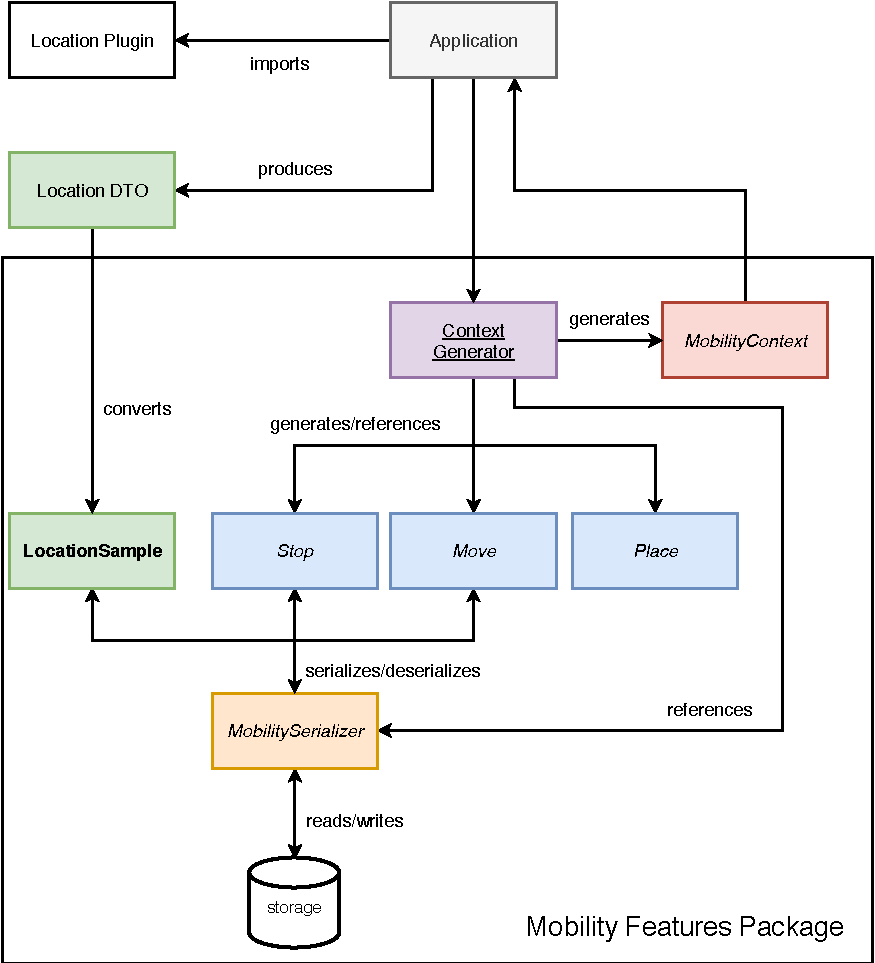
\includegraphics[width=0.5\textwidth]{images/diagrams/api-diagram.pdf}
    \caption{Component diagram for the Mobility Feature Package}
    \label{fig:component-diagram}
\end{figure}










\subsection{Main Algorithm}
For the package to work there needs to be a main algorithm which collected data, stored data on disk and computes the features when necessary. This algorithm is not implemented by the package itself, but rather by an application that uses the package. The reason for this is that the algorithm contains many steps which can be done in many ways according to what the application programmer is already using. For example, if an application programmer uses a local SQLite database to store other data, then it is ideal to use this database for storing the location data and intermediate features as well.

\begin{figure}
    \centering
    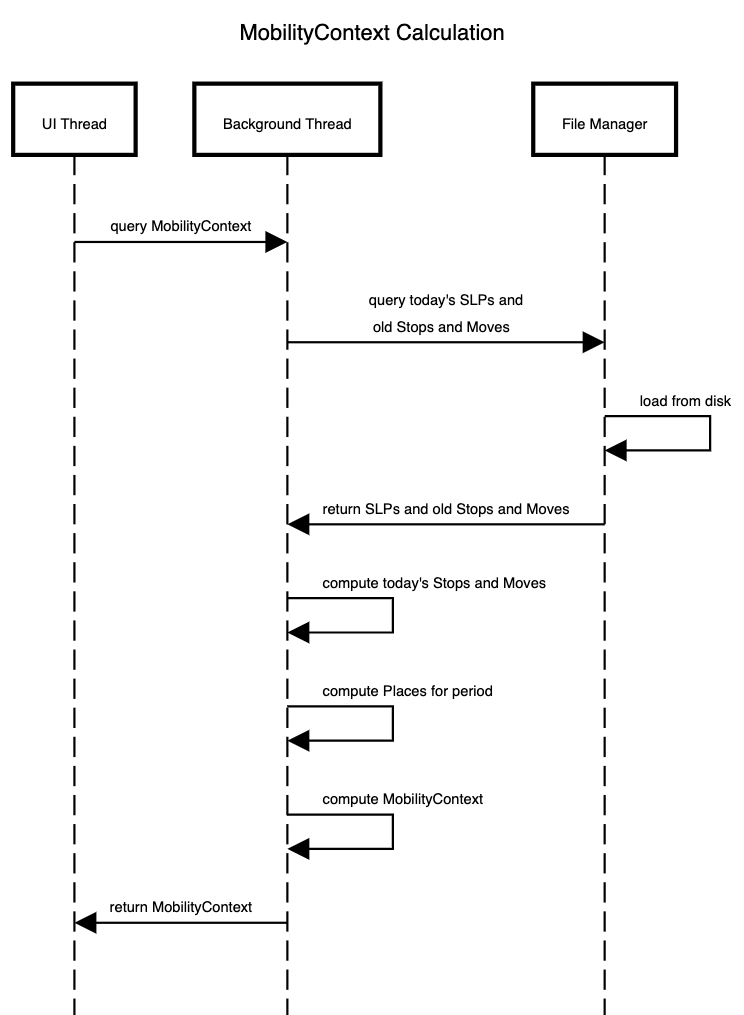
\includegraphics[width=0.7\textwidth]{images/diagrams/sequence.png}
    \caption{Sequence diagram for the computation of the Mobility Context in a mobile application}
    \label{fig:sequence-diagram-mobility-context}
\end{figure}
